\documentclass[12pt]{../SOP3_beta}\usepackage[]{graphicx}\usepackage[]{color}
%% maxwidth is the original width if it is less than linewidth
%% otherwise use linewidth (to make sure the graphics do not exceed the margin)
\makeatletter
\def\maxwidth{ %
  \ifdim\Gin@nat@width>\linewidth
    \linewidth
  \else
    \Gin@nat@width
  \fi
}
\makeatother

\definecolor{fgcolor}{rgb}{0.345, 0.345, 0.345}
\newcommand{\hlnum}[1]{\textcolor[rgb]{0.686,0.059,0.569}{#1}}%
\newcommand{\hlstr}[1]{\textcolor[rgb]{0.192,0.494,0.8}{#1}}%
\newcommand{\hlcom}[1]{\textcolor[rgb]{0.678,0.584,0.686}{\textit{#1}}}%
\newcommand{\hlopt}[1]{\textcolor[rgb]{0,0,0}{#1}}%
\newcommand{\hlstd}[1]{\textcolor[rgb]{0.345,0.345,0.345}{#1}}%
\newcommand{\hlkwa}[1]{\textcolor[rgb]{0.161,0.373,0.58}{\textbf{#1}}}%
\newcommand{\hlkwb}[1]{\textcolor[rgb]{0.69,0.353,0.396}{#1}}%
\newcommand{\hlkwc}[1]{\textcolor[rgb]{0.333,0.667,0.333}{#1}}%
\newcommand{\hlkwd}[1]{\textcolor[rgb]{0.737,0.353,0.396}{\textbf{#1}}}%
\let\hlipl\hlkwb

\usepackage{framed}
\makeatletter
\newenvironment{kframe}{%
 \def\at@end@of@kframe{}%
 \ifinner\ifhmode%
  \def\at@end@of@kframe{\end{minipage}}%
  \begin{minipage}{\columnwidth}%
 \fi\fi%
 \def\FrameCommand##1{\hskip\@totalleftmargin \hskip-\fboxsep
 \colorbox{shadecolor}{##1}\hskip-\fboxsep
     % There is no \\@totalrightmargin, so:
     \hskip-\linewidth \hskip-\@totalleftmargin \hskip\columnwidth}%
 \MakeFramed {\advance\hsize-\width
   \@totalleftmargin\z@ \linewidth\hsize
   \@setminipage}}%
 {\par\unskip\endMakeFramed%
 \at@end@of@kframe}
\makeatother

\definecolor{shadecolor}{rgb}{.97, .97, .97}
\definecolor{messagecolor}{rgb}{0, 0, 0}
\definecolor{warningcolor}{rgb}{1, 0, 1}
\definecolor{errorcolor}{rgb}{1, 0, 0}
\newenvironment{knitrout}{}{} % an empty environment to be redefined in TeX

\usepackage{alltt}
\usepackage[english]{babel}
%\usepackage{blindtext}
%\usepackage{lipsum}

%\documentclass{article}

%\documentclass[12pt]{~/github/SOPs/SOP_Template/SOP}

\title{Eureka Manta2 Multiprobe for water testing}
\date{10/30/2017}
\author{Haley Land-Miller}
\approved{Los Huertos}
\ReviseDate{\today}
\SOPno{21 v0.5}
\IfFileExists{upquote.sty}{\usepackage{upquote}}{}
\begin{document}

\maketitle

\section{Scope and Application}

\NP This SOP describes the procedures for calibrating and using the Eureka Manta2 Sub2 Multiprobe.

\NP This probe tests temperature, pH, depth, conductivity, and dissolved oxygen (in both g/L and \%). pH, conductivity, and dissolved oxygen all require calibration.

\NP The probe can be used to take the above measurements in bodies of water, including lakes, streams, and rivers. 

\section{Summary of Method}

\NP Calibration of any of the sensors is performed by selecting ``Standardize" from the Manta2 menu on the Amphibian portable PC and pouring standards into the calibration cup.

\NP Measurments are taken by connecting the probe to the Amphibian portable PC, placing the weighted protective cap over the sensors, and dropping the probe into the water being tested. 

\tableofcontents

\section{Definitions}

\NP Probe = the entire Manta2 apparatus that includes the five sensors.

\NP Sensor = one of the detectors on the probe, including those for temperature, pH, conductivity, dissolved oxygen, and the reference electrode.

\section{Interferences}

\NP Calibration is important for getting any meaningful data. 

\NP The reference electrode needs to be maintained by refilling the reference electrolytes once every few months. Not doing this can cause pH readings to be unreliable. 

\NP When using the probe in streams or rivers, take downstream measurments first to avoid your movements and presence affecting the measurments. For the same reason, stand on the bank or downstream of where you're taking the measurements while the probe is in the water.  

\section{Health and Safety}

\subsection{Safety and Personnnel Protective Equipment}

\NP Gloves should be worn when using the probe in bodies of water, because water may be contaminated. 

\NP Water shoes are useful for protecting your feet if you're planning to walk in the body of water while using the probe, which you will likely do. 

\section{Personnel \& Training Responsibilities}

Researchers using this SOP should be trained for the following SOPs:

\begin{itemize}
  \item SOP03 Field Work
  %\item SOP04 Electrical Power in the Field
\end{itemize}

\section{Required Materials}

\NP {Eureka Manta2 Sub2 probe}

\NP {Amphibian 2 portable PC}

\NP {Amphibian 2 charging cable}

\NP {Cable to connect Manta2 probe and Amphibian}

\NP {Standards for calibration (pH 4.00, 7.00, 10.00, conductivity, and a small bottle that can be used to make the DO standard)}

\section{Estimated Time}

\NP Charging the Amphibian 2 portable PC takes a fair amount of time - allow at least several hours, or leave it charging over night. 

\NP Calibration requires 20 minutes, if you're calibrating all sensors, and must be completed before going to the field.

\NP Site visits and data collection is relatively rapid, but the probe should be in the water for 2 minutes before a reading is taken. In addition, to get GPS readings, the GPS should be enabled 5 minutes before the reading.

\NP Cleaning the probe takes less than 5 minutes.

\section{Pre-field Preparation}

\subsection{Charging}

\NP Charge the Amphibian 2 portable PC before going into the field. The charger plugs into the round hole on the bottom edge of the Amphibian. 

\subsection{Calibration}

\NP Calibration of each sensor requires similar procedures. Set up your probe by removing the blue plug and covering it with a plastic protector. Insert the underwater cable in it's place to connect the Amphibian and the Manta. Turn on the Amphibian by pressing the power button on the bottom right corner. Press the Windows icon in the lower left corner. Scroll down to the bottom of the main page and select Amp\_2\_2\_6 \emph{or} use the short-cut button on the Amphibian numberpad \textbf{P1}. Once the interface loads, press ``Manta2" on the lower left bar, and select ``calibrate" from the menu that appears. Select the sensor you would like to calibrate. 

\NP Standardizing pH. To standardize the pH meter, follow the steps above and select ``pH units" from the Manta2 menu. The screen will instruct you to input the value of your first standard (pH) in the unshaded box. Then, unscrew just the blue cap from the larger cap of the probe, leaving the clear plastic cup surrounding the sensors in place. Pour a small amount of the first standard into the cup (with the probe facing upward), place the lid on, and shake, to rinse sensors in the standard. Do this twice in total and then fill the cup with 1 inch of the first standard. Once the red line on the chart of the Amphibian has stabalized (is coming out flat), press ``Ok". The screen will now prompt you to put in your second standard. Rinse and shake twice with DI water, and then twice with your second standard, before filling it above the sensors and repeating your process from above. When prompted, select the option to do a three-point calibration, and repeat these steps (including two rinses with DI and then with the standard) with your third standard. You have just set a "calibration curve."

\NP Calibrating the other sensors is very similar. Conductivity is a one-point calibration with one standard. For dissolved oxygen, pour tap water into a small bottle, about half full. Shake the bottle vigorously for several minutes, incorporating as much air as possible into the water. Go through the steps to start calibration of HDO, and pour the water into the cup. For dissolved oxygen, the sensor needs to be stable for 3 minutes before you press ``Ok". 

\section{Field Procedure}

\NP Connecting the Manta. Connect and power on the Manta to the Amphibian Portable PC as before. Adjust screen brightness using short-cut buttons \textbf{arrow up + P3} and \textbf{arrow up + P4}. When you open the Amp\_2\_2\_6, the Main screen will appear(A) (Figure~\ref{fig:AmphibianMain.png}). This is where you will see data readings. To log, or store, one line of data take a "snapshot" with the top left button (A). To locate snapshots, open the PDA menu in the bottom left corner and select "snapshot locations"(B). In the SS locations screen (C) you can edit your files or create a new one. When creating a new file (D), annotate using the guidelines in 10.5.To see data presented graphically, open the PDA menu and select "graphing" (B). To exit the program, again open the PDA menu and select "Exit."

\begin{figure}[h]
\centering
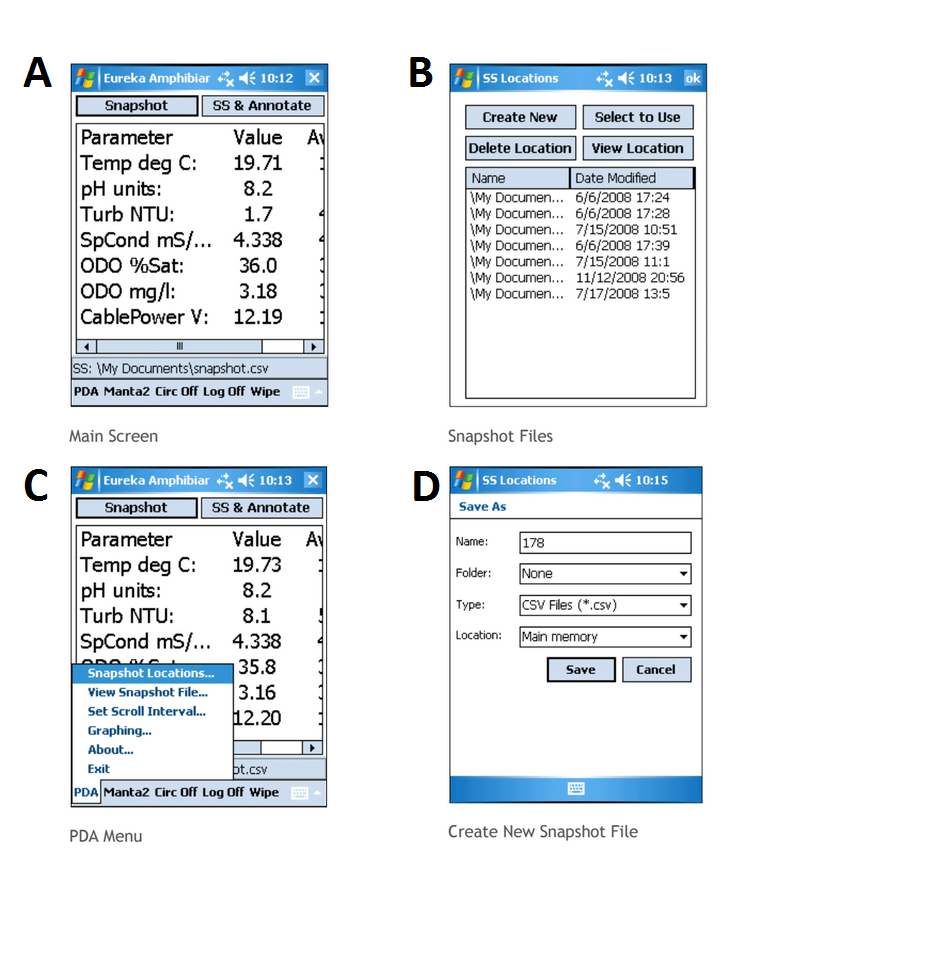
\includegraphics[scale=0.6]{AmphibianMain.png}
\caption{Amphibian Working Screens}
\label{fig:AmphibianMain.png}
\end{figure}

\NP Enable GPS. To turn on GPS, tap on the GPS/GNSS status gadget (Figure~\ref{2}). A satellite icon will appear on the bar across the top. While the amphibian is searching for satellites, it is important not to cover the top "cap" which holds the antenna as this will interfere with accuracy. Once satellites are found, information similar to that in the image below will appear.

\begin{figure}[h]
\centering
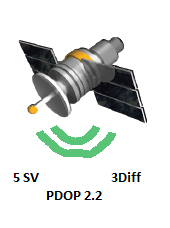
\includegraphics{GPS.png}
\caption{GPS Icon}
\label{GPS.png}
\end{figure}

\textbf{5 SV} Number of satellites used for the current position

\textbf{3Diff} 3 Satellites will create a 2D fix, 4 Satellites are required for a 3D fix.

\textbf{PDOP 2.2} A measure of Accuracy- the lower the number, the more accurate the fix is.

\NP Short-cut buttons. Remembering the short-cut buttons will save you lots of time in the field. 

{P1} - Opens the Amp\_2\_2\_6 app

{P2} - Opens short-cut buttons menu

{Up arrow + P3} - Brightness down

{Up arrow + P4} - Brightness up

{Camera Icon} - Camera

\NP Snap-shot and Annotation. In the Main Menu (A), the top right button allows you to screenshot and name your file simultaneously. Annotate using the following guidelines: Year.Month.Day.Project / Ex: 2017.10.2.pH

\NP Disconnecting the Manta. Disconnect the underwater cable from the probe and insert the blue storage plug. Be sure to cover the appropriate end of the underwater cable with the plastic protector. 

\section{Post-Field Procedures}

\NP Cleaning the Manta2. Clean the probe with warm soapy water. Liquid dishwashing soap or mild household cleaners work well. Clean sensor stems with a soft brush. Rinse well with tap water and \textbf{store sensors with tap water inside cup}.

\NP Downloading Data. Connect the Amphibian to your PC using a USB cord. A green window will open on your computer monitor with four options. Select "File Management." Another window will pop up, with a harddrive called "\" and within that, several folders. Select the folder "My Documents." Find the Excel document with your information.

\section{Trouble Shooting}

\NP Check for lights. The Manta2's green LED light indicates that it has sufficient voltage for usage. If you are still not getting enough voltage, try another cord.

\section{Advanced Use Options}

 \NP Autonomous data logging. In addition to using "snapshots" to capture data, you can activate an automatic "Logging" feature which records data at customized time intervals. See page 48 in the Manta2 Manual.

\section{References}

\NP APHA, AWWA. WEF. (2012) Standard Methods for examination of water and wastewater. 22nd American Public Health Association (Eds.). Washington. 1360. pp. (2014).

\end{document}
